
In allgemeinen Worten abgefasst ist Google-Polymer ein Framework, das sämtliche Funktionen von Web-Components zur Verfügung stellt. Polymer verfolgt den Ansatz, dass alles was entwickelt wird, eine Web-Komponente ist und sich mit der Entwicklung des Webs weiterentwickelt. Abbildung \ref{fig:3_polymer_architecture} auf Seite \pageref{fig:3_polymer_architecture} zeigt die Architektur von Polymer.


\begin{figure}[h]
\centering
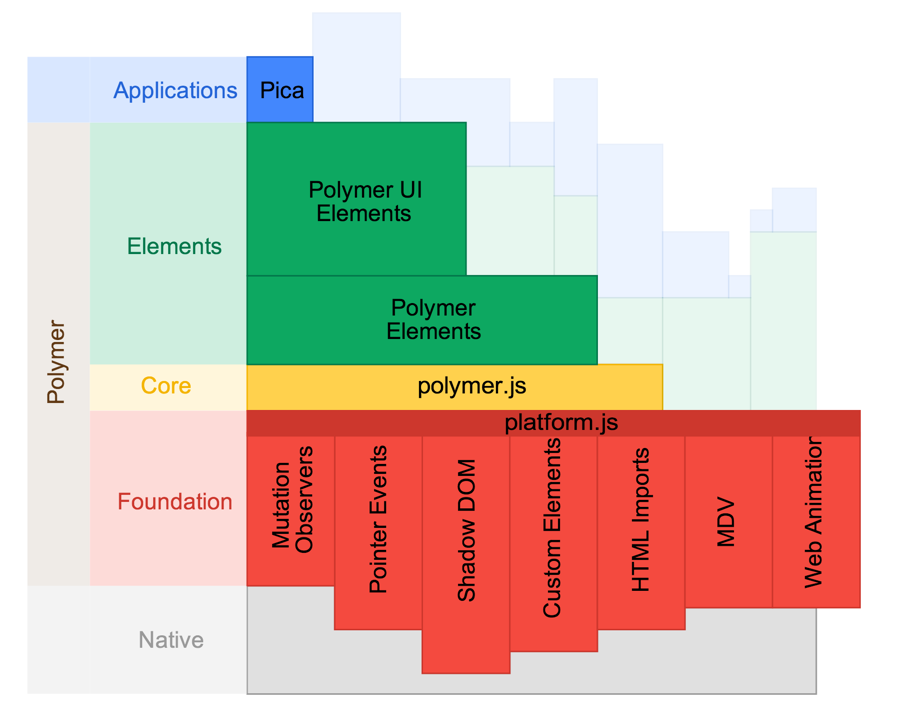
\includegraphics[height=5.0cm]{images/polymer_architecture.png}
\caption[
Polymers Architektur, Urldate: 04.2014 \newline
\small\texttt{http://www.polymer-project.org/images/architecture-diagram.svg}
]{Polymers Architektur}
\label{fig:3_polymer_architecture}
\end{figure}

\begin{description}
\item[Die rote Schicht] visualisiert die Polyfills, die Polymer zur Verfügung stellt. Diese erlauben die Benutzung von Web-Components. Wichtig hierbei ist, dass die Größe dieser Polyfill-Bibliotheken mit der Weiterentwicklung der Browser abnimmt. Dies bedeutet, dass je mehr Funktionalität von der Spezifikation in den Browsern implementiert ist, desto kleiner sind die Polyfill-Bibliotheken. Der Idealfall für Polymer wäre, dass sämtliche Zusatzbibliotheken, die die nativen Browser-Funktionen emulieren, nicht mehr benötigt werden.
\item[Die gelbe Schicht] stellt die Meinung von Google dar, wie die spezifizierten Browser Schnittstellen zu Web-Components zusammen verwendet werden sollen. Zusätzlich zu den spezifizierten Technologien werden des Weiteren Fuktionalitäten wie \glqq data-bindings\grqq , \glqq change watcher\grqq , \glqq public properties\grqq , etc. bereitgestellt.
\item[Die grüne Schicht] repräsentiert eine umfassende Reihe von Interface-Komponenten. Diese entwickeln sich ständig weiter und basieren auf der gelben, sowie roten Schicht.
\end{description}

Polymer bietet neben der Erstellung von benutzerdefinierten Elementen auch die Möglichkeit vordefinierte Elemente zu verwenden. Ein Beispiel für ein vordefiniertes Element wäre das \lstinline|<polymer-ajax>|-Element. Es erscheint in erster Linie als nicht sehr nützlich, jedoch versucht es, einen Standard für Entwickler bereitzustellen, um Ajax-Requests zu erstellen beziehungsweise abzuwickeln. Dieses Element ist ähnlich zu folgender Funktion von jQuery: \lstinline{$.ajax()}\footnote{Mehr Information zur jQuery.ajax-Funktion unter \href{http://api.jquery.com/jQuery.ajax/}{http://api.jquery.com/jQuery.ajax/}}. Der Unterschied zwischen den beiden Möglichkeiten einen Ajax-Request abzuwickeln ist, dass die \lstinline{$.ajax()}-Methode Abhängigkeiten besitzt, wohingegen die \lstinline|<polymer-ajax>|-Methode vollkommen unabhängig ist.

Wie man benutzerdefinierte Elemente mittels Polymer entwickelt und welche Coding-Conventions dieses Framework beinhaltet, wird in Kapitel \ref{sec:4_WC_Polymer} auf Seite \pageref{sec:4_WC_Polymer} genauer erläutert.